\documentclass[border=6pt]{standalone}
\usepackage{lmodern}
\usepackage[T1]{fontenc}
\usepackage{amsmath}
\usepackage{xcolor}
\usepackage{tikz}
\usetikzlibrary{arrows.meta}
\definecolor{cgray}{HTML}{8A8880}
\definecolor{cblue}{HTML}{2F7DC8}
\definecolor{cred}{HTML}{C0392B}
\definecolor{cgreen}{HTML}{4E8E2A}
\definecolor{cink}{HTML}{2B2B2B}
\tikzset{>={Stealth[length=2.2mm]},crv/.style={line width=1.0pt,smooth,samples=120}}
\newcommand{\gw}[1]{2.0*exp(0-(#1*#1)/5.12)} % true compatible residuals, sd 1.6
\newcommand{\gn}[1]{2.0*exp(0-(#1*#1)/2.0)}  % model-assumed scale, sd 1.0
\begin{document}
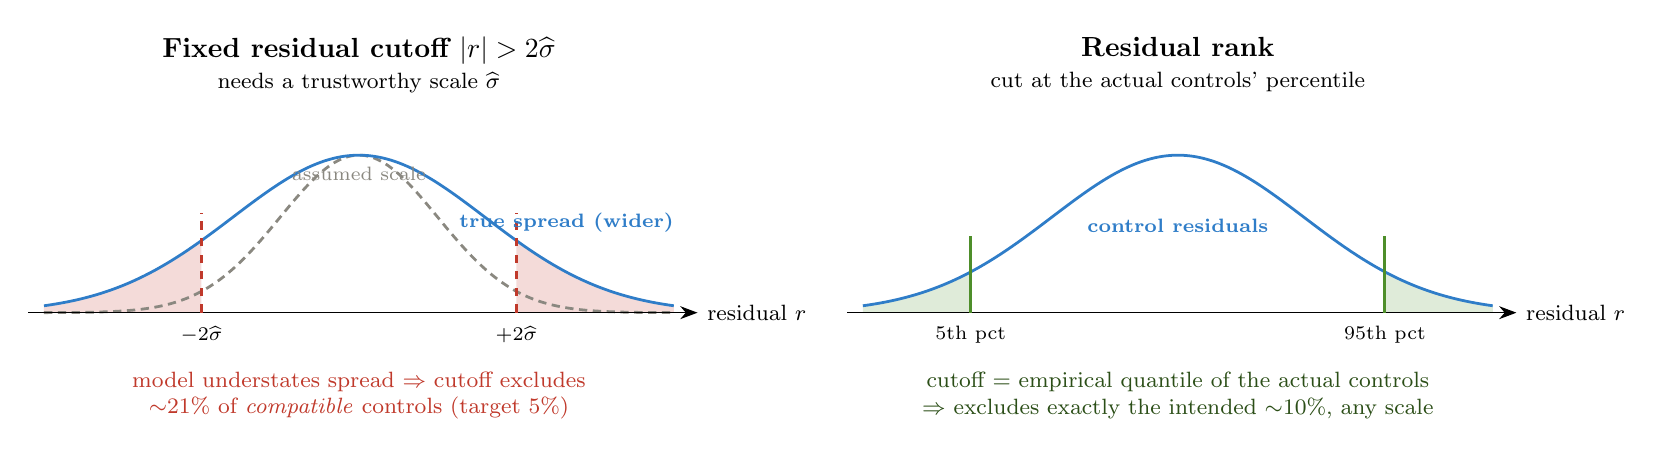
\begin{tikzpicture}[font=\small]

% ===== Panel A: fixed residual cutoff (fragile) =====
\begin{scope}
  \node[font=\bfseries,align=center] at (0,3.15) {Fixed residual cutoff $|r|>2\widehat\sigma$ \\[-1pt]\footnotesize\mdseries needs a trustworthy scale $\widehat\sigma$};
  % shade true-density mass beyond +/-2 (wrongly excluded)
  \fill[cred!18] (2.0,0) -- plot[domain=2.0:4.0,samples=40] (\x,{\gw{\x}}) -- (4.0,0) -- cycle;
  \fill[cred!18] (-4.0,0) -- plot[domain=-4.0:-2.0,samples=40] (\x,{\gw{\x}}) -- (-2.0,0) -- cycle;
  \draw[cgray,densely dashed,crv] plot[domain=-4:4] (\x,{\gn{\x}});
  \draw[cblue,crv] plot[domain=-4:4] (\x,{\gw{\x}});
  \draw[->] (-4.2,0) -- (4.3,0) node[right,font=\footnotesize]{residual $r$};
  \draw[cred,dashed,line width=1.0pt] (2.0,0) -- (2.0,{\gw{2.0}+0.35});
  \draw[cred,dashed,line width=1.0pt] (-2.0,0) -- (-2.0,{\gw{-2.0}+0.35});
  \node[below,font=\scriptsize] at (2.0,-0.05){$+2\widehat\sigma$}; \node[below,font=\scriptsize] at (-2.0,-0.05){$-2\widehat\sigma$};
  \node[cgray,font=\scriptsize,anchor=south] at (0.0,1.55) {assumed scale};
  \node[cblue,font=\scriptsize\bfseries,anchor=south west] at (1.15,0.9) {true spread (wider)};
  \node[cred,font=\footnotesize,align=center,text=cred] at (0,-1.05)
     {model understates spread $\Rightarrow$ cutoff excludes\\ $\sim$$21\%$ of \emph{compatible} controls (target $5\%$)};
\end{scope}

% ===== Panel B: residual rank (self-calibrating) =====
\begin{scope}[xshift=10.4cm]
  \node[font=\bfseries,align=center] at (0,3.15) {Residual rank \\[-1pt]\footnotesize\mdseries cut at the actual controls' percentile};
  \fill[cgreen!18] (2.63,0) -- plot[domain=2.63:4.0,samples=40] (\x,{\gw{\x}}) -- (4.0,0) -- cycle;
  \fill[cgreen!18] (-4.0,0) -- plot[domain=-4.0:-2.63,samples=40] (\x,{\gw{\x}}) -- (-2.63,0) -- cycle;
  \draw[cblue,crv] plot[domain=-4:4] (\x,{\gw{\x}});
  \draw[->] (-4.2,0) -- (4.3,0) node[right,font=\footnotesize]{residual $r$};
  \draw[cgreen,line width=1.1pt] (2.63,0) -- (2.63,{\gw{2.63}+0.45});
  \draw[cgreen,line width=1.1pt] (-2.63,0) -- (-2.63,{\gw{-2.63}+0.45});
  \node[below,font=\scriptsize] at (2.63,-0.05){$95$th pct}; \node[below,font=\scriptsize] at (-2.63,-0.05){$5$th pct};
  \node[cblue,font=\scriptsize\bfseries,anchor=south] at (0,0.9) {control residuals};
  \node[cgreen!55!black,font=\footnotesize,align=center] at (0,-1.05)
     {cutoff $=$ empirical quantile of the actual controls\\ $\Rightarrow$ excludes exactly the intended $\sim$$10\%$, any scale};
\end{scope}

\end{tikzpicture}
\end{document}
